\documentclass[10pt, a4paper]{article}
\usepackage[utf8]{inputenc}
\usepackage{mathtools}
\usepackage{array}
\usepackage[italian]{babel}
\usepackage[pdfusetitle]{hyperref}
\usepackage{cancel}
\usepackage{xcolor}
\usepackage[pdftex]{graphicx}
\usepackage{caption}
\usepackage{titling}
\usepackage{comment}

\title{Il formulario bellino}
\author{Lorenzo Cauli}

\setlength{\footskip}{90pt}
\setlength{\droptitle}{-10em}
\graphicspath{./images/}


\begin{document}
    \maketitle
    \hspace{-35pt}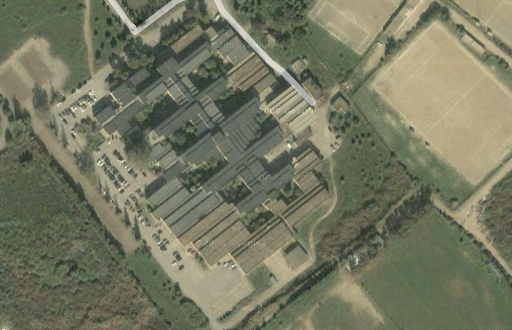
\includegraphics[width=400pt]{images/scano.png}
    \newpage
    \tableofcontents

    \newpage
    \part{Derivate}
    \section{Funzioni Razionali}
    \begin{center}
        \noindent\makebox[\textwidth]{
            \label{tab:derivate:razionali}
            \begin{tabular}{ |p{5em}|p{5em}|p{5em}|p{7em}|p{5cm}| }
                \hline
                Nome & Formula & Derivata & Esempio & Nota \\
                
                \hline
                
                % funzioni costanti
                \begin{center}
                    Costante
                \end{center} &
                \begin{align}
                    y=n \nonumber
                \end{align}  &
                \begin{align}
                    y'=0 \nonumber
                \end{align} &
                {
                    \begin{align}
                        y &= 4   \nonumber \\
                        y' & = 0 \nonumber 
                    \end{align}
                } &
                \begin{center}
                    La derivata di qualsiasi funzione costante equivale a 0 
                \end{center} \\ 

                \hline
                
                % razionali intere
                \begin{center}
                    Intera
                \end{center} &
                \begin{align}
                    y=x^n \nonumber
                \end{align} &
                \begin{align}
                    y'=nx^{n-1} \nonumber
                \end{align} &
                {
                    \begin{align}
                        y  & = 5x^2        \nonumber \\
                        y' & =(2*5)x^{2-1} \nonumber \\
                           & =10x          \nonumber
                    \end{align}
                } &  \\

                \hline
                
                % razionali frazionarie
                \begin{center}
                    Frazionaria
                \end{center} &
                \begin{align}
                    y = \frac{n}{x} \nonumber
                \end{align} &
                \begin{align}
                    y'=nx^{n-1} \nonumber
                \end{align} &
                \begin{center}
                    ---
                \end{center} &
                \begin{center}
                    Vedere "Rapporto" sezione \nameref{tab:derivate:operazioni} a pagina \pageref{tab:derivate:operazioni} \\
                \end{center}  \\
                \hline
            \end{tabular}
        }
    \end{center}
    \section{Funzioni Irrazionali}
    \begin{center}
        \noindent\makebox[\textwidth]{
            \label{tab:derivate:irrazionali}
            \begin{tabular}{ |p{5em}|p{5em}|p{5em}|p{7em}|p{5cm}| }
                \hline
                Nome & Formula & Derivata & Esempio & Nota \\
                
                \hline
                
                % funzioni costanti
                \begin{center}
                    Radice quadrata
                \end{center} &
                \begin{align}
                    y=\sqrt{x} \nonumber
                \end{align}  &
                \begin{align}
                    y'=\frac{1}{ 2\sqrt{x} } \nonumber
                \end{align} &
                {
                    \begin{align}
                        y  &= \sqrt{x^4}   \nonumber \\
                           &= x^\frac{4}{2}  \nonumber \\
                        y' &= \frac{\cancel{4}^2}{\cancel{2}_1}x^{\frac{\cancel{4}^2}{\cancel{2}_1}-1} \nonumber \\
                           &= 2x^{2-1} \nonumber \\
                           &= 2x \nonumber 
                    \end{align}
                } &
                \begin{center}
                    La radice quadrata puo' essere espressa come potenza, quindi si puo' applicare la regola per le funzioni razionali intere.
                \end{center} \\ 

                \hline
                
            \end{tabular}
        }
    \end{center}
    \section{Funzioni Esponenziali}
    \begin{center}
        \noindent\makebox[\textwidth]{
            \label{tab:derivate:esponenziali}
            \begin{tabular}{ |p{5em}|p{5em}|p{5em}|p{7em}|p{5cm}| }
                \hline
                Nome & Formula & Derivata & Esempio & Nota \\
                
                \hline
                
                % funzioni costanti
                \begin{center}
                    Funzione esponenziale
                \end{center} &
                \begin{align}
                    y=n^x \nonumber
                \end{align}  &
                \begin{align}
                    y'=n^xln(n) \nonumber
                \end{align} &
                {
                    \begin{align}
                        y  &= \sqrt{x^4}   \nonumber \\
                           &= x^\frac{4}{2}  \nonumber \\
                        y' &= \frac{\cancel{4}^2}{\cancel{2}_1}x^{\frac{\cancel{4}^2}{\cancel{2}_1}-1} \nonumber \\
                           &= 2x^{2-1} \nonumber \\
                           &= 2x \nonumber 
                    \end{align}
                } &
                \begin{center}
                    La radice quadrata puo' essere espressa come potenza, quindi si puo' applicare la regola per le funzioni razionali intere.
                \end{center} \\ 

                \hline
                
            \end{tabular}
        }
    \end{center}
    \section{Funzioni Logaritmiche}
    \begin{center}
        \noindent\makebox[\textwidth]{
            \label{tab:derivate:logaritmiche}
            \begin{tabular}{ |p{5em}|p{5em}|p{5em}|p{7em}|p{5cm}| }
                \hline
                Nome & Formula & Derivata & Esempio & Nota \\
                
                \hline
                
                % funzioni costanti
                \begin{center}
                    Logaritmo
                \end{center} &
                \begin{align}
                    y=\log_a{x} \nonumber
                \end{align}  &
                \begin{align}
                    y'=\frac{1}{x}\log_a{e} \nonumber
                \end{align} &
                {
                    \begin{align}
                        y  &= \sqrt{x^4}   \nonumber \\
                           &= x^\frac{4}{2}  \nonumber \\
                        y' &= \frac{\cancel{4}^2}{\cancel{2}_1}x^{\frac{\cancel{4}^2}{\cancel{2}_1}-1} \nonumber \\
                           &= 2x^{2-1} \nonumber \\
                           &= 2x \nonumber 
                    \end{align}
                } &
                {
                \begin{center}
                    Se il logaritmo ha come base \emph{e} (quindi si tratta di logaritmo naturale), la formula si puo' contrarre. \\
                    Esempio: \\
                    \begin{align}
                        y &= \ln{x} \nonumber \\
                        y' &= \frac{1}{x} \nonumber
                    \end{align}
                \end{center}
                } \\

                \hline
                
            \end{tabular}
        }
    \end{center}
    \section{Funzioni Goniometriche}
    \section{Operazioni tra funzioni}
    \begin{center}
        \noindent\makebox[\textwidth]{
            \label{tab:derivate:operazioni}
            \begin{tabular}{ |p{5em} | p{5em} | p{5em} | p{7em} | p{2cm}| }
                \hline
                Nome & Formula & Derivata & Esempio & Nota \\
                
                \hline
                
                % somma funzioni
                \begin{center}
                    Somma
                \end{center} &
                \begin{align}
                    y= {\color{red}f(x)} + {\color{blue}g(x)} \nonumber
                \end{align}  &
                \begin{align}
                    y'= {\color{red}f'(x)} + {\color{blue}g'(x)} \nonumber
                \end{align} &
                {
                    \begin{align}
                        y  &= {\color{red}x^2} + {\color{blue}4}   \nonumber \\
                        y' &= {\color{red}2x^{2-1}} + {\color{blue}0} \nonumber \\
                           &= 2x \nonumber 
                    \end{align}
                } &
                \begin{center}
                \end{center} \\ 

                \hline
                
                % differenza funzioni
                \begin{center}
                    Differenza
                \end{center} &
                \begin{align}
                    y= {\color{red}f(x)} - {\color{blue}g(x)} \nonumber
                \end{align}  &
                \begin{align}
                    y'= {\color{red}f'(x)} - {\color{blue}g'(x)} \nonumber
                \end{align} &
                {
                    \begin{align}
                        y  &= {\color{red}x^2} - {\color{blue}4}   \nonumber \\
                        y' &= {\color{red}2x^{2-1}} - {\color{blue}0} \nonumber \\
                           &= 2x \nonumber 
                    \end{align}
                } &
                \begin{center}
                \end{center} \\ 

                \hline
                
                % prodotto funzioni
                \begin{center}
                    Prodotto
                \end{center} &
                \begin{align}
                    y= {\color{red}f(x)} * {\color{blue}g(x)} \nonumber
                \end{align}  &
                \begin{align}
                    y'= ({\color{red}f'(x)} * {\color{blue}g(x)} ) + ( {\color{red}f(x)} * {\color{blue}g'(x)}) \nonumber
                \end{align} &
                {
                    \begin{align}
                        y  &= {\color{red}x^2} * {\color{blue}4}   \nonumber \\
                        y' &= ( {\color{red}2x^{2-1}} * {\color{blue}4} ) + ( {\color{red}x^2} * {\color{blue}0} ) \nonumber \\
                           &= (2x * 4) + 0 \nonumber \\
                           &= 8x \nonumber 
                    \end{align}
                } &
                \begin{center}
                \end{center} \\ 

                \hline
                
                % rapporto funzioni
                \begin{center}
                    Rapporto
                \end{center} &
                \begin{align}
                    y= \frac{\color{red}f(x)}{\color{blue}g(x)} \nonumber
                \end{align}  &
                \begin{align}
                    y'= \frac{[{\color{red}f'(x)} * {\color{blue}g(x)} ] - [ {\color{red}f(x)} * {\color{blue}g'(x)}]}{[{\color{blue}g'(x)}]^2} \nonumber
                \end{align} &
                {
                    \begin{align}
                        y  &= \frac{\color{red}x^2}{\color{blue}4}   \nonumber \\
                        y' &= \frac{( {\color{red}2x^{2-1}} * {\color{blue}4} ) - ( {\color{red}x^2} * {\color{blue}0} )}{{\color{blue}4}^2} \nonumber \\
                           &= \frac{({\color{red}2x} * {\color{blue}4}) - 0}{16} \nonumber \\
                           &= \frac{\cancel{8}^1x}{\cancel{16}_2} \nonumber  \\
                           &= \frac{x}{2} \nonumber
                    \end{align}
                } &
                \begin{center}
                \end{center} \\ 

                \hline
                
                % funzioni composte
                \begin{center}
                    Funzioni composte
                \end{center} &
                \begin{align}
                    y= {\color{red}f({\color{blue}g(x)})} \nonumber
                \end{align}  &
                \begin{align}
                    y'= {\color{red}f'({\color{blue}g(x)})} * {\color{blue}g'(x)} \nonumber
                \end{align} &
                {
                    \begin{align}
                        y  &= {\color{red}sin({\color{blue}2x^2})}   \nonumber \\
                        y' &= {\color{red}cos({\color{blue}2x^2})} * {\color{blue}4x} \nonumber 
                    \end{align}
                } &
                \begin{center}
                \end{center} \\ 

                \hline
                
            \end{tabular}
        }
    \end{center}

    \newpage
    \part{Integrali}
    \section{AAAA}
    \huge{WIP}

\end{document} 